\chapter{FUNDAMENTAÇÃO TEÓRICA}
Neste capítulo, são apresentados os principais conceitos e fundamentos necessários para a compreensão, 
entendimento e progresso deste trabalho.


\section{Séries Temporais}
    Muitas pessoas, em algum momento, já imaginaram como seria prever o futuro e ter acesso a informações sobre eventos 
    ou situações de suas vidas. Essa curiosidade reflete um desejo universal, mas também uma necessidade presente em 
    diversas áreas, como na gestão governamental, no setor financeiro e em contextos sociais. Nesse cenário, surge o 
    conceito de Série Temporal, definido como um conjunto de observações organizadas sequencialmente no tempo, 
    representadas por \( x_t \), com cada valor correspondente a um instante específico \(t\)~\cite{box2015}. O estudo de 
    Séries Temporais permite não apenas compreender as características de fenômenos que evoluem ao longo do tempo, mas 
    também desenvolver e ajustar modelos estatísticos capazes de explicar ou prever o comportamento dos dados 
    observados.
    
    De acordo com~\cite{brockwell2002}, séries temporais podem ser classificadas 
    discretas e continuas, uma série temporal é discreta quando o conjunto \( t_0 \) de tempos em que as observações 
    são feitas é um conjunto discreto, como o caso de observações que são realizadas em um determinado intervalo de 
    tempo fixo. Sendo representada por:
    \begin{equation}
        T = \{t_1, \dots, t_n\}, \quad \{X_t : t \in T\}
    \end{equation}
    
    
    E seríes temporais continuas quando suas observações são obtidas continualmente 
    no tempo. Sendo expressa por: 
    \begin{equation}
        T = [t_1, t_2], \quad \{X(t) : t \in T\}
    \end{equation}
        
    \subsection{Estacionariedade}
        A estacionariedade refere-se ao comportamento dos valores de uma série temporal ao longo do tempo. Uma série é 
        classificada como estacionária quando seus dados flutuam de maneira aleatória em torno de uma média fixa, mantendo-se em 
        um estado de equilíbrio ao longo do período analisado. Contudo, na prática, muitas séries temporais do cotidiano não 
        apresentam essa característica, exibindo tendências, sazonalidades ou outras formas de variação que indicam a presença de 
        não estacionariedade~\cite{morettin2018}.

    \subsection{Decomposição}

        \citeonline{costa2019} destaca que ao iniciar a análise de uma série temporal é de alta valia utilizar de gráficos 
        criados sequencialmente no tempo, visto que isso pode revelar determinados padrões de comportamento e algumas 
        características que podem estar presentes nos dados, como tendência, sazonalidade, ciclidade e ruído, também 
        conhecido como erro aleatório. 

        A tendência ($\mu_t$) apresenta um padrão de comportamento de grandezas em relação à variável tempo. De forma
        geral, elas revelam umc
        
        A ciclidade ($\psi_t$) pode ser \\
        
        A sazonalidade ($\gamma_t$) pode ser \\
        
        O ruído ($\epsilon_t$) é 

        %mostrar fórmulas

    \subsection{Modelos}


\section{Redes Neurais}
%Falar brevemente
    O cérebro humano é um sistema de grande complexidade, não linear e altamente paralelo, composto por cerca de 
    10 bilhões de neurônios. Cada neurônio está conectado, em média, a outros 10 bilhões de neurônios, formando uma 
    vasta e sofistiada rede. Na estrutura de um neurônio, destaca-se o corpo celular, também chamado de soma, que é 
    responsável por integrar os sinais recebidos. Os neurônios possuem canais de entrada, chamados dendritos, que 
    recebem informações de outros neurônios, e canais de saída, chamados axônios, que transmitem essas informações. 
    Os dendritos são considerados as "zonas receptivas" do neurônio, enquanto os axônios funcionam como 
    "linhas de transmissão".

    Os neurônios se comunicam por meio de sinais eletroquímicos. Os dendritos recebem essas informações de outros 
    neurônios através dos axônios. Quando o conjunto de sinais recebidos é suficientemente forte para ativar o 
    neurônio, este gera um impulso elétrico que percorre seu axônio. Esse sinal eletroquímico coordena e organiza a 
    atividade neuronal, permitindo ao cérebro realizar diversas formas de processamento de maneira extremamente 
    eficiente, muitas vezes mais rápida do que os computadores digitais convencionais~\cite{haykin2009neural}.

    A Figura \ref{fig:celula_piramidial} mostra a estrutura do neurônio:
    \begin{figure}[!htb]
        \centering
        \caption{Célula piramidial.}
        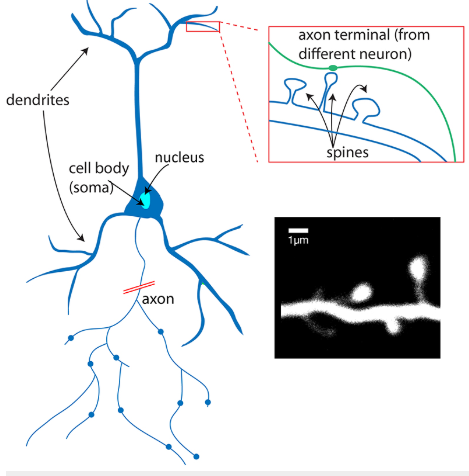
\includegraphics[scale=0.5]{celula-piramidial.png}\\
        {\footnotesize Fonte: The University Of Queensland.}\
        \label{fig:celula_piramidial}
    \end{figure}
    
    Ao entender de forma simples o poder de processamento que o ce
    \subsection{Histórico}
        As redes neurais são frequentemente consideradas um complemento à computação tradicional. Curiosamente, 
        John von Neumann, amplamente reconhecido como o pai da computação moderna devido à sua proposta da arquitetura 
        que possibilitou a criação do computador de programa armazenado, demonstrava grande interesse em modelar o 
        funcionamento do cérebro humano. Esse interesse levantou debates entre pesquisadores sobre a possível interação 
        entre as ideias de von Neumann e os primórdios das redes neurais. Alguns estudiosos destacam indícios que 
        sugerem a visão de von Neumann sobre as direções futuras do desenvolvimento dos computadores~\cite{Fausett1994}.

        Neste capítulo, serão destacados alguns marcos significativos que tiveram um papel fundamental no avanço e
        desenvolvimento da área de redes neurais.


        \subsubsection{Perceptrons}
            
            Em 1958, o psicólogo Frank Rosenblatt publicou um artigo que, pela primeira vez, descreveu de forma 
            algorítmica o funcionamento de um modelo de rede neural para aprendizagem supervisioanda. Essa 
            publicação inspirou inúmeros pesquisadores a direcionarem seus esforços para estudos sobre redes neurais, 
            explorando diversos aspectos dessa temática ao longo das décadas de 1960 e 1970~\cite{haykin2009neural}.

            \begin{figure}[!htb]
                \centering
                \caption{Fluxo do perceptron.}
                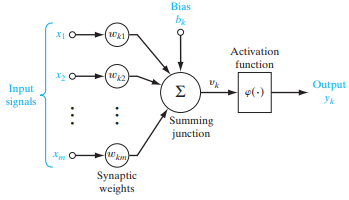
\includegraphics[scale=0.8]{fluxo-perceptron.png}\\
                {\footnotesize Fonte: Haykin (2009).}\
                \label{fig:fluxo-perceptron}
            \end{figure}

            Como apresentado na Figura~\ref{fig:fluxo-perceptron}, o perceptron consiste de um único neurônio com 
            pesos sinápticos ajustáveis e um viés. Ele possui uma camada de entrada (a retina) conectada aos pesos e 
            uma camada de saída. Seu funcionamento baseia-se em um combinador linear seguido por uma função de 
            ativação que realiza uma função linear. Esse nó somador (o neurônio) calcula uma combinação linear das 
            entradas aplicadas às suas sinapses, além de incorporar um viés aplicado externamente que ajusta a posição
            da função de ativação. O resultado dessa soma é passado à função de ativação, que produz uma saída de +1 
            se a entrada for positiva, ou -1, se for negativa. 
            
            O perceptron é um classificador binário, pois resolve apenas problemas de classificação de padrões 
            linearmente separáveis, ou seja, é capaz de lidar exclusivamente com problemas nos quais duas classes 
            podem ser separadas por uma linha em um hiperplano~\cite{haykin2009neural}. 


        % \subsubsection{Adaline}

        %     Em 1960, Bernard Widrow e Marcian Hoff desenvolveram uma regra de aprendizagem denominada "Regra Delta", 
        %     também conhecida como Least Mean Squares (LMS) ou método do Gradiente Descendente. Com base nessa regra, 
        %     foi criada uma rede neural com a mesma estrutura do Perceptron, composta por uma camada de entrada, uma 
        %     camada de saída e um único neurônio. A diferença principal reside na regra de aprendizado empregada para 
        %     o ajuste dos pesos, enquanto o Perceptron ajusta os pesos com base na saída binária da rede, essa rede
        %     utiliza a diferença entre o previsto e real e aplica o gradiente descendente para reduzir o erro.
            
        %     A Regra Delta, que tem como finalidade ajustar os pesos do neurônio, busca minimizar a diferença entre a 
        %     saída desejada e a resposta obtida a partir da combinação linear de todas as amostras. Utilizando a 
        %     minimização do erro quadrático médio entre os valores previstos e reais, o método opera dentro de um 
        %     contexto de aprendizagem supervisionada, onde há uma saída esperada previamente definida. O algoritmo 
        %     ajusta iterativamente o vetor de pesos \( w\) atribuído à rede, com o objetivo de determinar um 
        %     \( w^{*} \) ótimo tal que o erro quadrático \({E(w{*})}\), calculado sobre todo o conjunto de amostras, 
        %     seja minimizado.

        %     Essa rede neural foi projetada para aplicações em sistemas de chaveamento de circuitos telefônicos e 
        %     ficou conhecida como Adaline (Adaptive Linear Neuron). A Adaline foi uma das primeiras redes neurais 
        %     implementadas em contextos industriais, marcando um avanço significativo na aplicação de tecnologias 
        %     baseadas em inteligência artificial. Além disso, a regra de aprendizagem Widrow-Hoff para uma rede neural 
        %     de apenas uma camada foi o percursor da regra de Backpropagation para múltiplas camadas~\cite{Fausett1994,silva2010}
            
    \subsection{Componentes das Redes Neurais}
        % \subsubsection{Neurônio}
        % \subsubsection{Camadas}
        % \subsubsection{Função de Ativação}
        % \subsubsection{Função de Perda}
        % \subsubsection{Algoritmo de Otimização}
        % \subsubsection{Taxa de Aprendizado}


    \subsection{Processo de Treinamento}
        Sistemas de aprendizado de máquina podem ser categorizados de acordo com o tipo de treinamento que
        eles recebem. O aprendizado supervisionado ocorre quando o modelo é treinado por meio de exemplos explicítos. 
        Em contrapartida, no aprendizado não supervisionado, não há a definição de exemplos explicítos para orientar o 
        modelo. Além disso, existem diversas boas práticas para garantir que o modelo consiga realizar um bom aprendizado 
        e métricas para avalia-lo
         
        \subsubsection{Aprendizado Supervisionado e Não Supervisionado}  
        %Falar de forma breve o que é o aprendizado supervisionado e seus tipos
            No aprendizado supervisionado, o modelo é treinado com pares de dados \((x,y)\), onde \(x\) representa 
            os dados de entrada e \(y\) o valor esperado (ou rótulo). Durante o treinamento, o modelo compara as 
            previsões feitas com os valores reais utilizando uma função de perda, que mede o erro. Em seguida, 
            seus parâmetros são ajustados iterativamente, geralmente por meio de métodos como o gradiente descendente, 
            para minimizar esse erro e melhorar a precisão das previsões.
            
            No aprendizado não supervisionado, o modelo não recebe o par de dados \((x,y)\), mas apenas as entradas 
            \(x\). A partir disso, ele busca identificar padrões, estruturas ou associações presentes nos dados, 
            ajustando os pesos de acordo com o objetivo do método utilizado.

        
        \subsubsection{Pre-Processamento dos Dados}
            Antes de treinar um modelo com algoritmos de aprendizado de máquina, é imprescindível realizar o pré-processamento 
            dos dados. Esse processo assegura que os dados estejam padronizados, consistentes e adequados, permitindo que os 
            modelos alcancem um desempenho superior e resultados confiáveis nas métricas de avaliação. Para isso, são utilizadas 
            técnicas que evitam problemas como dados ausentes, inconsistências, valores conflitantes e incongruentes. Essas 
            técnicas são geralmente divididas em quatro categorias principais: limpeza, integração, transformação e redução de 
            dados~\cite{silva2021, oliveira2024}.

            \subsubsubsection{Limpeza de Dados}
                Um problema comum em conjuntos de dados (\emph{datasets}) é a presença de valores faltantes (ou nulos), que 
                podem ocorrer devido a diferentes fatores. Esses fatores incluem registros manuais realizados de forma 
                inadequada, falhas em sistemas de extração, transformação e carregamento de dados (\emph{ETL}) ou até mesmo 
                problemas em sensores de dispositivos autônomos. A presença de valores faltantes compromete tanto a qualidade 
                dos dados quanto o desempenho do treinamento de modelos de \emph{machine learning}, caso não seja tratada 
                adequadamente.~\citeonline{sivakumar2017} apresentam algumas abordagens eficazes para lidar com essa 
                problemática, como:

                \begin{itemize}
                    \item Exclusão de linhas do \emph{dataset} que contenham valores faltantes.
                    \item Preenchimento dos valores ausentes utilizando métricas estatísticas, como a média ou mediana, 
                    para gerar estimativas aproximadas que mantenham a coerência do conjunto de dados.
                \end{itemize}
                
            \subsubsubsection{Integração de Dados}
                É o processo de combinar dados provenientes de diversas fontes, ecossistemas e tecnologias, de maneira adequada 
                e coerente. Durante esse processo de integração, podem surgir problemas, como inconsistências nos dados e 
                redundâncias no conjunto de dados gerado~\cite{sivakumar2017, silva2021, oliveira2024}

            \subsubsubsection{Transformação de Dados}
                Nesse estágio, os dados são transformados em formatos adequados para utilização no modelo. 
                \citeonline{sivakumar2017} e \citeonline{oliveira2024} definem algumas atividades executadas nesta etapa:

                \begin{itemize} 
                    \item Uso de normalização para ajustar os valores dos dados a uma escala comum, permitindo fácil comparação entre 
                    diferentes atributos. 
                    \item Eliminação de ruídos com técnicas de suavização. 
                    \item Aplicação de técnicas de agregação para resumir dados complexos e detalhados. 
                    \item Generalização de valores específicos em categorias mais amplas, como, por exemplo, a generalização de 
                    faixas etárias. 
                \end{itemize}

            \subsubsubsection{Redução de Dados}
                Nessa etapa, são utilizadas metodos para reduzir o volume de dados que serão analisados, visando maior velocidade
                de processamento e melhora na eficiência do processo, mas sem comprometer a qualidade e integridade dos dados 
                originais.~\citeonline{sivakumar2017} indicam algumas estrategias, sendo elas:
                \begin{itemize}
                    \item Redução de dimensionalidade do \emph{dataset}, removendo atributos que não melhoram a perfomance do 
                    modelo.
                    \item Utilização de operações de agregação de dados para resumo de informações.
                    \item Utilização de técnicas de \emph{encoding} para compactação de dados.
                \end{itemize}

        \subsubsection{Overfitting e Undefitting}
        %Abordar sobre esses dois problemas, o que são, como surgem, como detectar e como se previnir

        \subsubsection{Técnicas de Validação}
        %Falar o que é, porque foi criada e modo de uso
        \subsubsubsection{Hold-Out}
        \subsubsubsection{K-Fold}
        \subsubsubsection{Leave-One-Out}
        \subsubsubsection{Bootstrap}

        \subsubsection{Métricas de Avaliação}
            Vide que a utilização de modelos de \emph{machine learning} é com o foco de predizer determinados eventos atráves
            de métodos estáticos e probabilisticos. A exatidão da previsão é o fator crucial em avaliar a qualidade de um modelo.
            \citeonline{sousa2011} apresenta a Tabela~\ref{fig:tabela-metricas} com as métricas mais comuns para avaliar as previsões
            dos modelos.
            
            \begin{center}
                \begin{table}[h!]
                    \centering
                    \caption{Cálculo de erros}
                    \label{tab:calculo_erros}
                    \begin{tabular}{ll}
                        \toprule
                        \textbf{Designação} & \textbf{Fórmula} \\ 
                        \midrule
                        Erro Absoluto Médio (MAE) & $\frac{1}{n} \sum_{t=1}^{n} |e_t|$ \\[8pt]
                        Erro Quadrático Médio (MSE) & $\frac{1}{n} \sum_{t=1}^{n} (e_t)^2$ \\[8pt]
                        Raiz do Erro Quadrático Médio (RMSE) & $\sqrt{\frac{1}{n} \sum_{t=1}^{n} (e_t)^2}$ \\[8pt]
                        Erro Percentual Absoluto Médio (MAPE) & $\frac{1}{n} \sum_{t=1}^{n} \left(\frac{|e_t|}{|y_t|}\right) 100$ \\ 
                        \bottomrule
                    \end{tabular}
                    
                    \bigskip
                    \small \textbf{Fonte:} Sousa (2011)
                    \label{fig:tabela-metricas}
                \end{table}
            \end{center}
            
            
    \subsection{Arquitetura}
    %Falar o que é e botar uma imagem em todas
        \subsubsection{Multi Layer Perceptron}            
            O algoritmo de backpropagation ajusta os pesos da rede neural para reduzir o erro entre a saída prevista 
            e o valor esperado. O erro é calculado e propagado pelas camadas até atingir um nível mínimo aceitável~\cite{marangoni2010}.
            
            \citeonline{grus2021} apresenta o funcionamento padrão do treinamento de uma rede neural utilizando o algoritmo 
            de backpropagation como método de ajuste dos pesos. Considera-se que a rede possui \( n\),  os quais são 
            ajustados de acordo com o seguinte procedimento:
            \begin{enumerate}
                \item Realiza-se o feed-forward, em que as entradas são processadas para produzir as saídas de todos os neurônios;
                \item Como o algoritmo é supervisionado, os valores esperados das saídas são conhecidos. Assim, calcula-se uma função de perda, geralmente definida como a soma dos erros quadráticos entre as saídas reais e as esperadas;
                \item O gradiente dessa função de perda é calculado em relação aos pesos dos neurônios de saída;
                \item Os gradientes e os erros são propagados para trás com o objetivo de calcular os gradientes associados aos pesos dos neurônios ocultos;
                \item Atualizam-se os pesos aplicando um passo em direção ao gradiente descendente, controlado por um parâmetro denominado learning rate (taxa de aprendizagem).
            \end{enumerate}
        \subsubsection{Redes Neurais Recorrentes}
        \subsubsection{Redes Neurais Convolucionais}
        \subsubsection{Long Short-Term Memory (LSTM)}
